%% 
%% Copyright 2007, 2008, 2009 Elsevier Ltd
%% 
%% This file is part of the 'Elsarticle Bundle'.
%% ---------------------------------------------
%% 
%% It may be distributed under the conditions of the LaTeX Project Public
%% License, either version 1.2 of this license or (at your option) any
%% later version.  The latest version of this license is in
%%    http://www.latex-project.org/lppl.txt
%% and version 1.2 or later is part of all distributions of LaTeX
%% version 1999/12/01 or later.
%% 
%% The list of all files belonging to the 'Elsarticle Bundle' is
%% given in the file `manifest.txt'.
%% 

%% Template article for Elsevier's document class `elsarticle'
%% with numbered style bibliographic references
%% SP 2008/03/01

%%\documentclass[preprint,10pt]{elsarticle}

%% Use the option review to obtain double line spacing
%% \documentclass[authoryear,preprint,review,12pt]{elsarticle}
%\documentclass[preprint,review,12pt]{elsarticle}
\documentclass[preprint,12pt]{elsarticle}

%% Use the options 1p,twocolumn; 3p; 3p,twocolumn; 5p; or 5p,twocolumn
%% for a journal layout:
%% \documentclass[final,1p,times]{elsarticle}
% %\documentclass[final,1p,times,twocolumn]{elsarticle}
% %\documentclass[final,3p,times]{elsarticle}
%% \documentclass[final,3p,times,twocolumn]{elsarticle}
%% \documentclass[final,5p,times]{elsarticle}
%% \documentclass[final,5p,times,twocolumn]{elsarticle}

%% For including figures, graphicx.sty has been loaded in
%% elsarticle.cls. If you prefer to use the old commands
%% please give \usepackage{epsfig}

%% The amssymb package provides various useful mathematical symbols
\usepackage{amssymb}
\usepackage{subfigure}
%% The amsthm package provides extended theorem environments
%% \usepackage{amsthm}

%% The lineno packages adds line numbers. Start line numbering with
%% \begin{linenumbers}, end it with \end{linenumbers}. Or switch it on
%% for the whole article with \linenumbers.
%% \usepackage{lineno}

\journal{Physics Letters B}
\input def.tex

\begin{document}

\begin{frontmatter}

\input frontpage.tex

%\begin{abstract}
%% Text of abstract

%\end{abstract}

%%\begin{keyword}
%% keywords here, in the form: keyword \sep keyword

%% PACS codes here, in the form: \PACS code \sep code

%% MSC codes here, in the form: \MSC code \sep code
%% or \MSC[2008] code \sep code (2000 is the default)

%%\end{keyword}

\end{frontmatter}

\linenumbers
\setcounter{tocdepth}{2}
\tableofcontents

%% main text
%\section{}
%\label{}
%---
\section{Introduction}\label{sec:intro}\label{sec:introduction}

\dsf\ is a Liquid Argon Time Projection Chamber (\lar\ \tpc), operated in Italy's Gran Sasso National Laboratory (LNGS) to search for nuclear recoils induced by weakly interacting massive particles (WIMPs). The first physics result was reported in \cite{Agnes:2015gu} based on 50 live data collection days with Atmospheric Argon (AAr), providing the most sensitive limit on a dark matter search using a \lar\ \tpc\ to date with a 90\% CL upper limit on the WIMP-nucleon spin-independent cross section of $6.1 x 10^{-44}$ cm$^2$ for a WIMP mass of 100 GeV/c$^2$.  %along with two other key results: ar bg can be suppressed for ton-scale experiments using \uar and efficiency of the veto 

A first WIMP search using argon extracted from underground sources (Underground Argon, UAr) has been reported in \cite{Agnes:2015_uar}, following the WIMP search with AAr. UAr has a lower concentration of the radioactive $\beta$-emitter $^{39}$Ar by a factor (1.4 $\pm$ 0.2) $\times\, 10^3$ relative to AAr. Calibration campaigns have been performed in the presence of AAr and UAr.

\dsf\ apparatus is described in detail in \cite{Agnes:2015gu}. As shown in fig.~\ref{fig:wholeAssembly_insideDetectors} it features a \lar\ \tpc\ surrounded by a 30 t liquid scintillator-based veto (LSV) system, placed inside a water Cerenkov veto detector (\wcv), both which measure in-situ and suppress radiogenic and cosmogenic backgrounds. On \wcv's top is a radon-free clean room (CRH) housing the cryogenic supply system and electronics (Fig.~\ref{fig:CALIS_photos}). The \lsv's inside is accessible from CRH through four access ports called organ pipes closed by gate valves. 

%After this introduction the CALIS design requirements and hardware realization are described in Sec.~\ref{sec:hardware}. Calibration campaigns and some of their physics highlights are discussed in Sec.~\ref{sec:CalibCampaigns}, before concluding in Sec.~\ref{sec:Conclusion}.

\begin{figure}[htbp]
 \centering
\includegraphics[width=\textwidth]{Figures/DS50_with_CALIS}
\caption{A conceptual drawing of CALIS (1) installed in radon-free clean room CRH (2) atop water Cerenkov veto (\wcv, 3) and with deployment device (4) containing the source deployed in liquid scintillator veto (LSV, 5) next to liquid argon time projection chamber's (\lar\ \tpc) cryostat (6). Clean room and LSV are connected through four access ports called organ pipes (only one of which is drawn in above sketch: (7)). All four organ pipes end in CRH at gate valves (8) which can be manually opened or closed. During normal operations all four organ pipes are closed. Not included in sketch are tubes connecting cryogenic systems in CRH to cryostat in \lsv\ \cite{Agnes:2015qyz}.\label{fig:wholeAssembly_insideDetectors}\label{fig:DS50_with_CALIS}}
\end{figure}

\begin{figure}[htbp]
 \centering
\subfigure{\includegraphics[width=0.335\textwidth]{./Figures/CALISinCRH_PetersComment.png}}
\subfigure{\includegraphics[width=0.52\textwidth]{./Figures/Next2Cryostat_80cm.png}}
\caption{\textit{left}: CALIS after installation inside radon-free clean room CRH. The organ pipe is 80 cm off-center with respect to TPC's vertical z-axis. \textit{right}: Photograph taken with a camera looking upwards into \lsv\ from the bottom. It shows source deployment device deployed through one of the organ pipes visible on top right. The arm is articulated and source is next to \lar\ \tpc's cryostat \cite{Agnes:2015qyz}.
\label{fig:CALIS_photos}}
\end{figure}

\subsection*{Laser calibration}
\wcv, \lsv\ and \tpc\ electronics gain calibration is performed with dedicated Laser systems, in place in each of three subdetectors. \wcv\ laser calibration is sufficient to veto muons (and their secondaries) with high efficiency. \tpc\ detector response has been calibrated using the internal ${39}$Ar and $83m$Kr, that has been added into \lar\ recirculation system during dedicated calibration campaigns \cite{Agnes:2015gu}.



%time line plot, how did the veto change during the calibration campaigns - allowing for systematics studies.
%table on what was the goal of each campaign. What sources were used


%safety requirements

%design section
%installation: before, after


\section{Design Requirements \& Hardware Implementation} \label{sec:hardware}\label{sec:design_requirements}

\subsection{Hardware}
The apparatus consists of the housing, which has been installed in CRH (Fig.~\ref{fig:CALIS_photos}, left) and the deployment device which can be lowered into the LSV (Fig.~\ref{fig:CALIS_photos}, right). The deployment device is attached to the housing through two stainless steel cables that are wound up on cable spools (Fig.~\ref{fig:CALISMechanism}).

\subsubsection{Deployment \& Articulation}\label{sec:DeploymentArticulation}
The center of the \lsv\ is about 6 m below the gate valve inside CRH
%=6145=70+120+400+3455+20+251+1372+457 from http://darkside-docdb.fnal.gov:8080/cgi-bin/RetrieveFile?docid=858&filename=NoFlyZone-DS50_vers02.pdf&version=14
 and the $6''$ wide organ pipes are vertical, yet about 80 cm off center in the XY plane as shown in Fig.~\ref{fig:CALIS_photos}. For \tpc\ calibration the radioactive source has to be positioned in immediate contact with the cryostat, in order to minimize rate losses through absorption in particular for low energy sources such as $^{57}$Co (122 keV). This is made possible by enabling the deployment device to articulate an arm, at whose end the radioactive source is thereby brought close the cryostat. 

\begin{figure}[htbp]
 \centering
 %\subfigure{ \includegraphics[width=0.7\textwidth]{Figures/gearDrawing}}
 \includegraphics[width=0.72\textwidth]{Figures/CALISDimensions.png}
 \includegraphics[width=0.27\textwidth]{Figures/CALIS_overview_IMG_3763.jpg}
 \caption{%\textit{top}:Looking down on the top of CALIS III and inside the upper assembly: the components and drive mechanism are shown. The hand wheel is on the left connected to one of the spools only. The next parts going from left to right are the two cable spools and then the sealed motor housing.
Mechanical drawing of CALIS showing the housing and the deployment device. Dimensions are in inches. (The total height of 88.75 inches corresponds to 225.425 cm.) The two modes of operation are illustrated: In order to move the deployment device downinto the LSV or back up the stepper motor moves both cable spools simultaneously. \textcolor{blue}{In order to articulate, the articulation wheel is rotated manually, which affects only the left spool, thereby shortening the left cable wrt.~to the right cable thereby articulating the arm and lifting the pivot center.} The amount of lifting and the amount of rotations until a horizontal articulation is reached has been calibrated prior to installation in CRH (Sec.~\ref{sec:Testing:LNGS})\label{fig:CALISDimensions}\label{fig:CALISMechanism}\label{fig:gearDrawing}
}
\end{figure}

In order to send the deployment device into the LSV, both cables are unwound simultaneously. The stepper motor moves both cable spools concurrently and an absolute encoder monitors the current position of the deployment device. The stepper motor is controlled via a simple graphical LabVIEW interface, run on a dedicated laptop, in which the current z-position is shown and a target z-position can be provided by the operator. Z-positions are given in motor step counts, an arbitrary unit which has been calibrated outside CRH in meters (Fig.~\ref{fig:z_test}) and relative to the TPC using the t-drift distribution of calibration data (Fig.~\ ref{fig:SourcePosition}, p.~\pageref{fig:SourcePosition}).

\begin{figure}[htbp]
 \centering
 \includegraphics[width=3.2in]{Figures/Z_positioning_test}
 \caption{Plot of the z position of the pig vs the step position of the motor.}
 \label{fig:z_test}
\end{figure}

Articulation of the arm is done manually via the articulation wheel (Fig.~\ref{fig:CALISMechanism}). This affects only the cable spool close to the articulation wheel, the left one in Fig.~\ref{fig:CALISMechanism}, thereby shortening the left cable wrt.~to the right cable and engaging the gear through a chain (Fig.~\ref{fig:sourceArmRotation}). As a result the arm is articulated and the pivot center is lifted. The degrees corresponding to a horizontal articulation has been calibrated prior to installation in CRH (Sec.~\ref{sec:Testing:LNGS}).

%The deployment and articulation mechanism involving two steel cables

%From testing.tex
(...) This is necessary because, as the cable winds around the spool, the winding radius changes, increasing as the pig is lifted and decreasing as it is lowered.  This means that there is not a linear correspondence between the number of steps and the length of cable deployed.  Additionally, this non-linear dependency causes the amount of rotation required by the hand wheel for full articulation of the source arm to change as a function of the length of cable deployed.     


Articulation and a movement in z-direction are mutually exclusive since the articulation of the arm leads to more wound up cable on the spool close to the articulation wheel wrt.~the other. If then in deployment mode both spools would be rotated simultaneously with the same angular speed, the cable close to the articulation wheel would wind up faster than the other, which would lead to a build up of difference in cable length and the deployment device would only be hanging on one cable. In order to avoid an imbalanced z-movement the arm has to be dearticulated before a change in z-position can be initiated. This is enforced by an electric switch preventing z-movement, which is disengaged only when the arm is fully dearticulated. 

\begin{figure}[htbp]
 \centering
\begin{minipage}[b]{0.48\textwidth}
\centering
  \includegraphics[width=\textwidth]{Figures/SourcePod2_mirrored.jpg}
\end{minipage}
\begin{minipage}[b]{0.48\textwidth}
\centering
  \includegraphics[width=\textwidth]{Figures/sourceArmArticulation.png}
  \includegraphics[width=0.8\textwidth]{Figures/IMG_2457.JPG}
\end{minipage}
  \caption{Technical drawing showing the articulation mechanism using a chain that engages the gear to transfer the rotation of the articulation wheel (Fig.~\ref{fig:CALISMechanism}) into a rotation of the source arm. The chain has a guard rail, not shown in the drawing, that ensures that the chain can never come off the gear.}
  \label{fig:sourceArmRotation}
\end{figure} 

\subsubsection{Housing \& Scintillator}

Besides providing mechanical support for the deployment device, the housing is the important interface between CRH and the LSV, through which sources are exchanged, while protecting the liquid scintillator and avoiding human contact with the liquid scintillator. The liquid scintillator, which is a mixture of PC and TMB\footnote{As discussed in Sec.~\ref{sec:CalibCampaigns} the concentration of TMB has varied during the campaigns.} with the wavelength shifter PPO\cite{DS50:firstPaper}, may not get exposed to oxygen or water as is present in normal clean room air and also contamination with $^{222}$Rn and its daughters has to be avoided. Vacuum and nitrogen pressurization systems have been developed \ref{sec:N2_pressure_system}.

On the other hand TMB vapors and residues could form ...

\textit{ToDo: more precise on risks of contact of TMB with air/ water. What are the dangers compared to a PC only scintillator?}

The housing thereby has the same role as glove boxes in calibration devices of other experiments (see e.g.~\cite{KamLAND:Calib,Borexino:Calib}).

\subsection{Design Requirements}
The design of CALIS is shaped by the following requirements, thereby following the design principle of ``form follows function'': 
\begin{itemize}
\item to allow source exchanges and safely deploy them at various positions inside the LSV, 
\item protecting the scintillator from oxygen and water at any time, in particular during deployments and being able to articulate a source arm in order to bring the source next to the cryostat. Also protection and safety mechanisms that avoid exposure of personal to scintillators are in place.
\item To complement studies of nuclear recoils with neutron sources ($^{241}$Am$^{9}$Be and $^{241}$Am$^{13}$C), it is planned to deploy a neutron gun inside a dedicated deployment device currently under development (Section \ref{sec:Outlook}).
\item All materials that come in contact with the scintillator veto are made of stainless steel and teflon except for the sealing o-rings which are made out of viton.  All three materials (stainless steel, teflon, and viton) are certified materials for contact with TMB and PC.
\item Before assembly in CRH, each component of CALIS, the ones introduced into the scintillator as well as those in the clean room CRH, have been subjected to the official cleaning procedure \cite{DS50:cleaning}.
\end{itemize}

This results in further hardware design choices and requirements that are discussed below.
\subsection{Hardware Details}

\subsubsection{Housing}
%from bottom to top

Here the design of the housing shown in fig.~\ref{fig:CALISMechanism} is described in more detail. Starting at the gate valve inside the clean room CRH on which CALIS has been installed, a a teflon disk allows to electrically isolate CALIS from ground, even though during normal operations the CALIS housing is also connected to ground. A tripod with a bellow has been used to vertically align the housing right after installation on the gate valve. The bellow is connected to a 23.375" long cylindrical stainless steel enclosure pipe. It has the same diameter as the organ pipe (6'') and leads into a view port (depicted in blue in fig.~\ref{fig:CALISMechanism}) and which is the access point for accessing the source arm and exchanging sources.  

Above the view port is the upper assembly, which is a stainless steel cylindrical enclosure that houses the cable drive mechanism, including the cable spools the stepper motor and the articulation mechanism, already described in Sec.~\ref{sec:DeploymentArticulation}. 

CALIS offers various safety features to ensure that the device runs smoothly, no components are lost inside the detector, avoid any contamination of the detector by dirty or incompatible materials, maintain pressure and avoid introduction of oxygen or water in contact with the LS and TMB, operation in the volume that excludes possibility of contact with PMTs or light pulsers (pacman) attached to each PMT.
 
\subsubsection{Safety features}

\begin{description}

\item[Drive mechanism:]
The drive mechanism is a stepper motor that has an integrated absolute encoder providing the location of the source at all times, even in the event of a power failure. In the event of a power failure, the magnetic break ensures there is no movement of the pig. The torque of the servo motor is limited in case of an unexpected load. 

The speed reducer (gears) is a double worm gear design. The primary worm gear has a 50:1 reduction and the secondary worm has a 82:1 reduction. The input speed of the servo motor is 2400 RPMs and the output is 0.6 RPM and has the weight capacity of 148 lbs. In the event of a power failure the speed reducer has the ability to hold the load at any position without back drive. The speed of the motor has been limited to 0.4\,cm/s which minimizes any lateral oscillation of the pig during lowering and raising the source. Additionally, this is the maximum speed at which the motor is not overheating.

\item[Manual retraction system:]
In the unlikely case of a complete motor failure while the source is deployed, it is possible to manually retract the pig back to its home position and close the gate valve. The motor is disengaged, and wrench is used to manually wind the cable back onthe spools and retract the pig back above the gate valve. 

\item[Cable strength and length:]
The cables holding the pig have been rated for loads over 590\,kg, while the weight of the pig is at the level of 10-15\,kg so well below the breaking strength of the cable. The cable length has been established so that the maximum depth at which the pig can be deployed is above the level of the PMTs inside the LSV. In case, the command is given to deploy to greater depth, the cable completely unwinds and then rewinds in the opposite direction, which then effectively retracts the pig to a higher z-position until the preset motor count of steps is reached. 

%% is this true?

   
\item[Upper limit switch:]
The motor has an absolute encoder and step position is never lost even in the case when the motor loses power. When the pig has reached its home position within the upper assembly it will stop.  However, if the top of the pig continues past its home position (based on the number of steps given), it will not be able to pass its home position thanks to the upper limit switch that will be triggered in that case. 

Neither the manual retraction system has been used nor has the upper limit switch been activated during calibration campaigns.


     
\item[Light and leak tightness of CALIS:]
When the deployment device is next to the cryostat the gate valve is open and we take also data with the LSV. A prerequisite is that the housing is absolute light tight and pressure leak tight. All view ports have light tight covers for when the organ pipe gate valve is open. Both light and leak tightness has been extensively validated throughout the manufacturing process until including commissioning (Sec.~\ref{sec:Commissioning}).

\end{description}
	
%%%%%%%%%%%%%%%%%%%%%%%%%%%%%%%%%%%%%%%%%
%%%%%%%%%%%%%%%%%%%%%%%%%%%%%%%%%%%%%%%%%

\subsubsection{Deployment device}
The pig (Fig. \ref{fig:sourcePod_arrows}) contains the support structure for the arm which holds the source at its end.  This piece is equipped with tapered cones on the top and bottom that ensure that the ends do not get snagged on inner edges of the organ pipe as it is moving up and down. It is attached to the housing by two cables.  Swivel hooks are employed in the attachment of the cables to the pig that allow the cables to move freely and not get tangled. 
There are two weights built into the device, one cylindrical in the conical cap above the rotation gear mechanism and one inside the cones at the bottom end of the device. Both help to minimize any lateral motion or oscillations during deployment and articulation and dearticulation especially. It also ensures smooth motion of the deployment device into the organ pipe and back to the home position inside the housing.

\subsubsection{Source holder and arms}
A source arm and the source holder are attached to the articulation gear (Fig.~\ref{fig:SourceHolder}). Different arm lengths have been prepared with a maximum arm length of 62 cm, the arm length thereby being measured from the pivot point of the rotation gear to the tip of the source holder. This arm length allows the source to be placed in immediate contact with the cryostat (Fig.~\ref{fig:CALIS_photos}, right), as the center axis of the organ pipe is 81 cm from the TPC center and the cryostat has an outer radius of 32 cm. The 62 cm arm was used for most of the deployments in the past calibration campaigns (Sec.~\ref{sec:CalibCampaign}). Inside the source holder the radioactive source is placed, pressed to the tip and held in place via a spring during deployment, articulation and dearticulation. The source holder is sealed such that no liquid scintillator can enter during the deployment. This has also been verified during each source extraction, that no liquid was found on the inside.

\begin{figure}[htbp]
 \centering
  \includegraphics[width=0.7\textwidth]{Figures/SourceHolder.png}
  \caption{Source holder that connects to an arm and to the articulation gear of the deployment device. The source, here a $^{133}$Ba source is pressed to the tip of the source holder via a spring.}
  \label{fig:SourceHolder}
\end{figure}


\subsubsection{Securing of the source}
All connection points for the source and arm have been secured with two push locking pins that cannot be disengaged without a person pressing the pin. 
The source holder is held in place via a locking mechanism and two locking pins. When the source is attached to the arm, the source container must be slid over a protruding pin. There is a sliding locking mechanism that interlocks onto the pin. Once the source is locked into position there are 2 additional locking pins that are put into place (one above and one below the source holder pin), each of which have a button that must be depressed in order for the pins to be released. In addition, the source holder and the 2 locking pins will all be tethered from outside the view port until they are locked in place eliminating the possibility of accidental falling.  The tethering will happen before installation of the source and before the removal of the source. The cables used to tether the pins and the source holder during installation and removal will be detached after installation and prior to deployment to avoid the possibility of the arm getting entangled.  
 
%\begin{figure}[htbp]
 %\centering
% \includegraphics[width=3.2in]{Figs/sourceHolder_locking}
% \caption{Locking mechanism for the source holder. This photo shows two push pins that ensure that the sliding pin stays in place and the the source holder %cannot under any circumstances get detached from the arm.  The only way to remove the push pins is to depress buttons on each of them by hand. }
% \label{fig:sourceHolder_locking}
%\end{figure}

%\begin{figure}[htbp]
% \centering
 % \includegraphics[width=7in]{Figs/sourceAttachmentParts}
%  \caption{Components of the source attachment mechanism. Central image shows how the pin that holds the source holder slides down and prevents the %source from getting loose.  The slide pin is locked in place by two push pins shown in Fig. \ref{fig:sourceHolder_locking}}
%  \label{fig:sourceAttachmentParts}
%\end{figure}

\subsection{Degrees of freedom}

CALIS is capable of deploying sources at various positions inside the \lsv. Besides movement along Z up to its maximum cable length, it is possible to articulate at an angle of $\theta$ between 0$^{\circ}$ and 90$^{\circ}$, where $\theta$ is the zenith-angle (Fig.~\ref{fig:coordinate_system}). Angles of more than 90$^{\circ}$ are excluded because the articulation chain's end is reached at a 90$^{\circ}$ angle (see Fig.~\ref{fig:sourceArmRotation}).

\begin{figure}[htbp]
 \centering
  \includegraphics[height=0.35\textheight,clip=true]{Figures/DeploymentDevice_XY_view}
  \includegraphics[height=0.35\textheight]{Figures/CALIS_sideview_Cary.jpg}
  \caption{There are two degrees of freedom in the source deployment position after a certain source arm length has been chosen: \textit{Left}: The device can be rotated in the XY-plane by an angle $\phi$, except for the region excluded by the presence of the cryostat. In most cases the source has been in contact with the cryostat. 
\textit{Right:} Articulation to an angle $\theta$ between 0$^{\circ}$, when it is dearticulated, and 90$^{\circ}$, when the arm is horizontally articulated. During most calibration campaigns the source has been horizontal.
  \label{fig:coordinate_system}}
\end{figure} 
%https://en.wikibooks.org/wiki/LaTeX/Importing_Graphics on clip=true removes white space around the picture - neat!

\subsubsection*{XY-plane rotation}\label{sec:XYrotation}
A sealed connection below the view port has an o-ring seal and uses a ring clamp to compress the seal. This clamp can be slightly loosened allowing the upper assembly (everything above and including the view port) to be rotated with respect to the lower assembly and the \tpc. Rotation in the XY-plane can even be performed while the device is deployed next to the cryostat, since the seal is helium leak and light tight even when loosened.

In principle a rotation of 360$^\circ$ can be done, except when the arm would interfere with the cryostat. This has been used in one calibration campaign to deploy a neutron source directly next to the cryostat and rotated away ($\phi\,=\,90^\circ$) to study optical shadowing effects from the cryostat (Sec.~\ref{sec:CalibCampaigns}). 



%For articulation, there is currently a choice of three arm lengths---40.3\,cm,  57.15\,cm and 62\,cm.  
%Each of these lengths are measured from the center line of the organ pipe to the end of the source holder.  The arm lengths, 57.15\,cm and 62\,cm are intentionally made too long as they will be used to determine the exact location of the cryostat; some uncertainty in the cryostat's z and lateral position exist at the level of 3 - 4\,cm. The organ pipe we intend to use is 81\,cm distant from the cryostat center (and the geometric center of the LSV sphere) as measured from the center line of the organ pipe. The cryostat is 32\,cm in radius, which leaves a distance of $\sim$49\,cm to be reached  by the arm.


\begin{figure}[htbp]
 \centering
  \includegraphics[width=0.7\textwidth]{Figures/RingClamp_WithPin_IMG_2669.JPG}
%  \includegraphics[scale=0.5]{Figures/RingClamp.jpg}
  \caption{Beneath the view port is a ring clamp with a ruler underneath. The rotation angle is read from the ruler going around the pipe. The ruler is in mm, which has been calibrated in degrees. To perform azimuthal rotation, the ring clamp is slightly loosened, and the entire upper assembly is rotated with respect to the lower assembly, along with the deployment device.}
  \label{fig:ring_clamp}
\end{figure} 

\subsubsection*{``No fly'' zone}
A ``no fly'' zone is defined directly above the cryostat where there are many TPC supply tubes. No deployment device part may enter in this region, particularly the source arm.

%\begin{figure}[htbp]
% \centering
%  \includegraphics[scale=0.5]{Figures/NoFlyZone.png}
%  \caption{``No fly'' zone for the CALIS source arm.}
%  \label{fig:NoFlyZone}
%\end{figure} 

\subsubsection*{Default configuration}
By default, the deployment device has been deployed with the longest source arm (62 cm) in a horizontal position in contact with the cryostat, at the same height as the center of the TPC's active volume (Fig.~\ref{fig:coordinate_system}). 

Other degrees of freedom could involve shorter arm lengths, while longer arm lengths would require hardware modifications on the deployment device. Out of four organ pipes, a second one is available for source calibration. (Two organ pipes are not available due to interference with existing infrastructure: the cryogenic tower and the electronics rack.) Moving CALIS to a different organ pipe requires a partial disassembly of CALIS and reinstallation on the other organ pipe's gate valve.

%Finally CALIS is designed to house also a different deployment device, such as currently being planned for the neutron gun \cite{???}.
\section{Testing, Cleaning and Commissioning} \label{sec:Testing}\label{sec:Commissioning}
CALIS has been assembled at FNAL from components produced at FNAL and University of Hawaii. After initial basic functionality tests at FNAL, CALIS was shipped pre-assembled to LNGS, where it underwent a comprehensive testing and calibration program. While still outside clean room CRH, CALIS was installed on a high bay platform in the LNGS underground hall C and tested at its full length. Besides testing basic Z-motion, articulation and XY-rotation, all details of CALIS operations ranging from testing functionality of motor controls, high limit and articulation switch to recovery scenarios after e.g.~power failures during deployment were validated.

An important aspect was source's Z-position calibration as a function of cable length before and after source arm articulation, which is a nonlinear function of motor step counts, as mentioned in Sec.~\ref{sec:Nonlinearity:MotorStepCounts}. Furthermore source's XY- and Z-position accuracy and precision was estimated.

This testing campaign's results were reviewed by an internal review board and approval for installation inside CRH was granted. CALIS was cleaned according to official cleaning procedures and installed on gate valve in September 2014.
After installation on gate valve a testing focus was system's light and helium leak tightness, and nitrogen and vacuum systems testing, as these could only be tested fully after installation. A more detailed description of tests performed at FNAL and LNGS can be found in \cite{thesis:Hackett, thesis:Edkins}.

\subsection*{XY- and Z-position}
Tests in air and in \lsv's scintillator revealed source position accuracy and precision is dominated by uncertainties during articulation. Positioning in Z before articulation is highly accurate and precise: deployment speed is very low, barely visible to the naked eye (4 mm/s), which minimizes lateral motion during deployment and contact with housing or organ pipe is avoided during deployment. Yet during articulation a swing in XY arises from tiny laterally imbalanced forces originating in articulating cable pull. 

To ensure deployment precision a procedure has been worked out to make reliably gentle contact with the cryostat, thereby eliminating precision uncertainty in XY: After positioning deployment device in Z, source arm is articulated to horizontal while it is pointing away from the cryostat. Only then source is brought into contact with cryostat through a XY-rotation while monitoring photomultiplier tube (PMT) scaler rates, which increase while source is approaching, yet plateaus as soon as contact with the cryostat is made, even if XY-rotation continues. This provides a reliable XY- and Z-position for calibration source and was used throughout calibration campaigns.
%part of testing, cleaning and commissioning section

\subsection{Operational Procedure}
After the testing and commissioning CALIS has been installed inside CRH... 

Well, there also have been test deployments before that.
\subsubsection{Source Insertion}

\subsubsection{3 special positions}
home position or parking position - gate valve closed. The 

center of the TPC.

Full extension position - length of the cable.


\subsubsection{Vacuum evacuation (flushing) and nitrogen purging}
   One of the most important features of this system is making sure that the TMB and PC residue on the device are extracted from CALIS III prior to opening access ports to exchnage source or arms. This is  important for  safe working level of the people involved and for the detector.  This can be addressed through a system evacuation and nitrogen purge.  To accelerate the removal of the TMB in the scintillator fluid residue that is left after a deployment, CALIS III will undergo an evacuation with a vacuum pump. By lowering the pressure inside of CALIS below the vapor pressure of the TMB, it will cause the TMB to outgas and be removed through the vent line of the vacuum pump. An additional step to remove the TMB is to purge using N$_{2}$.  We will need to limit the potential flow rate of the nitrogen to ensure that an ODH (Oxygen Deficiency Hazard) condition is avoided in CRH.  Only once this is accomplished, will the view port be allowed to be opened and the source handled.     
  
The entire CALIS III  has been tested at FNAL  to hold pressure.  The system will be tested again after installation on the gate valve.
 

\begin{figure}[htbp]
 \centering
  \includegraphics[width=0.49\textwidth]{Figures/GasSystem.png}
  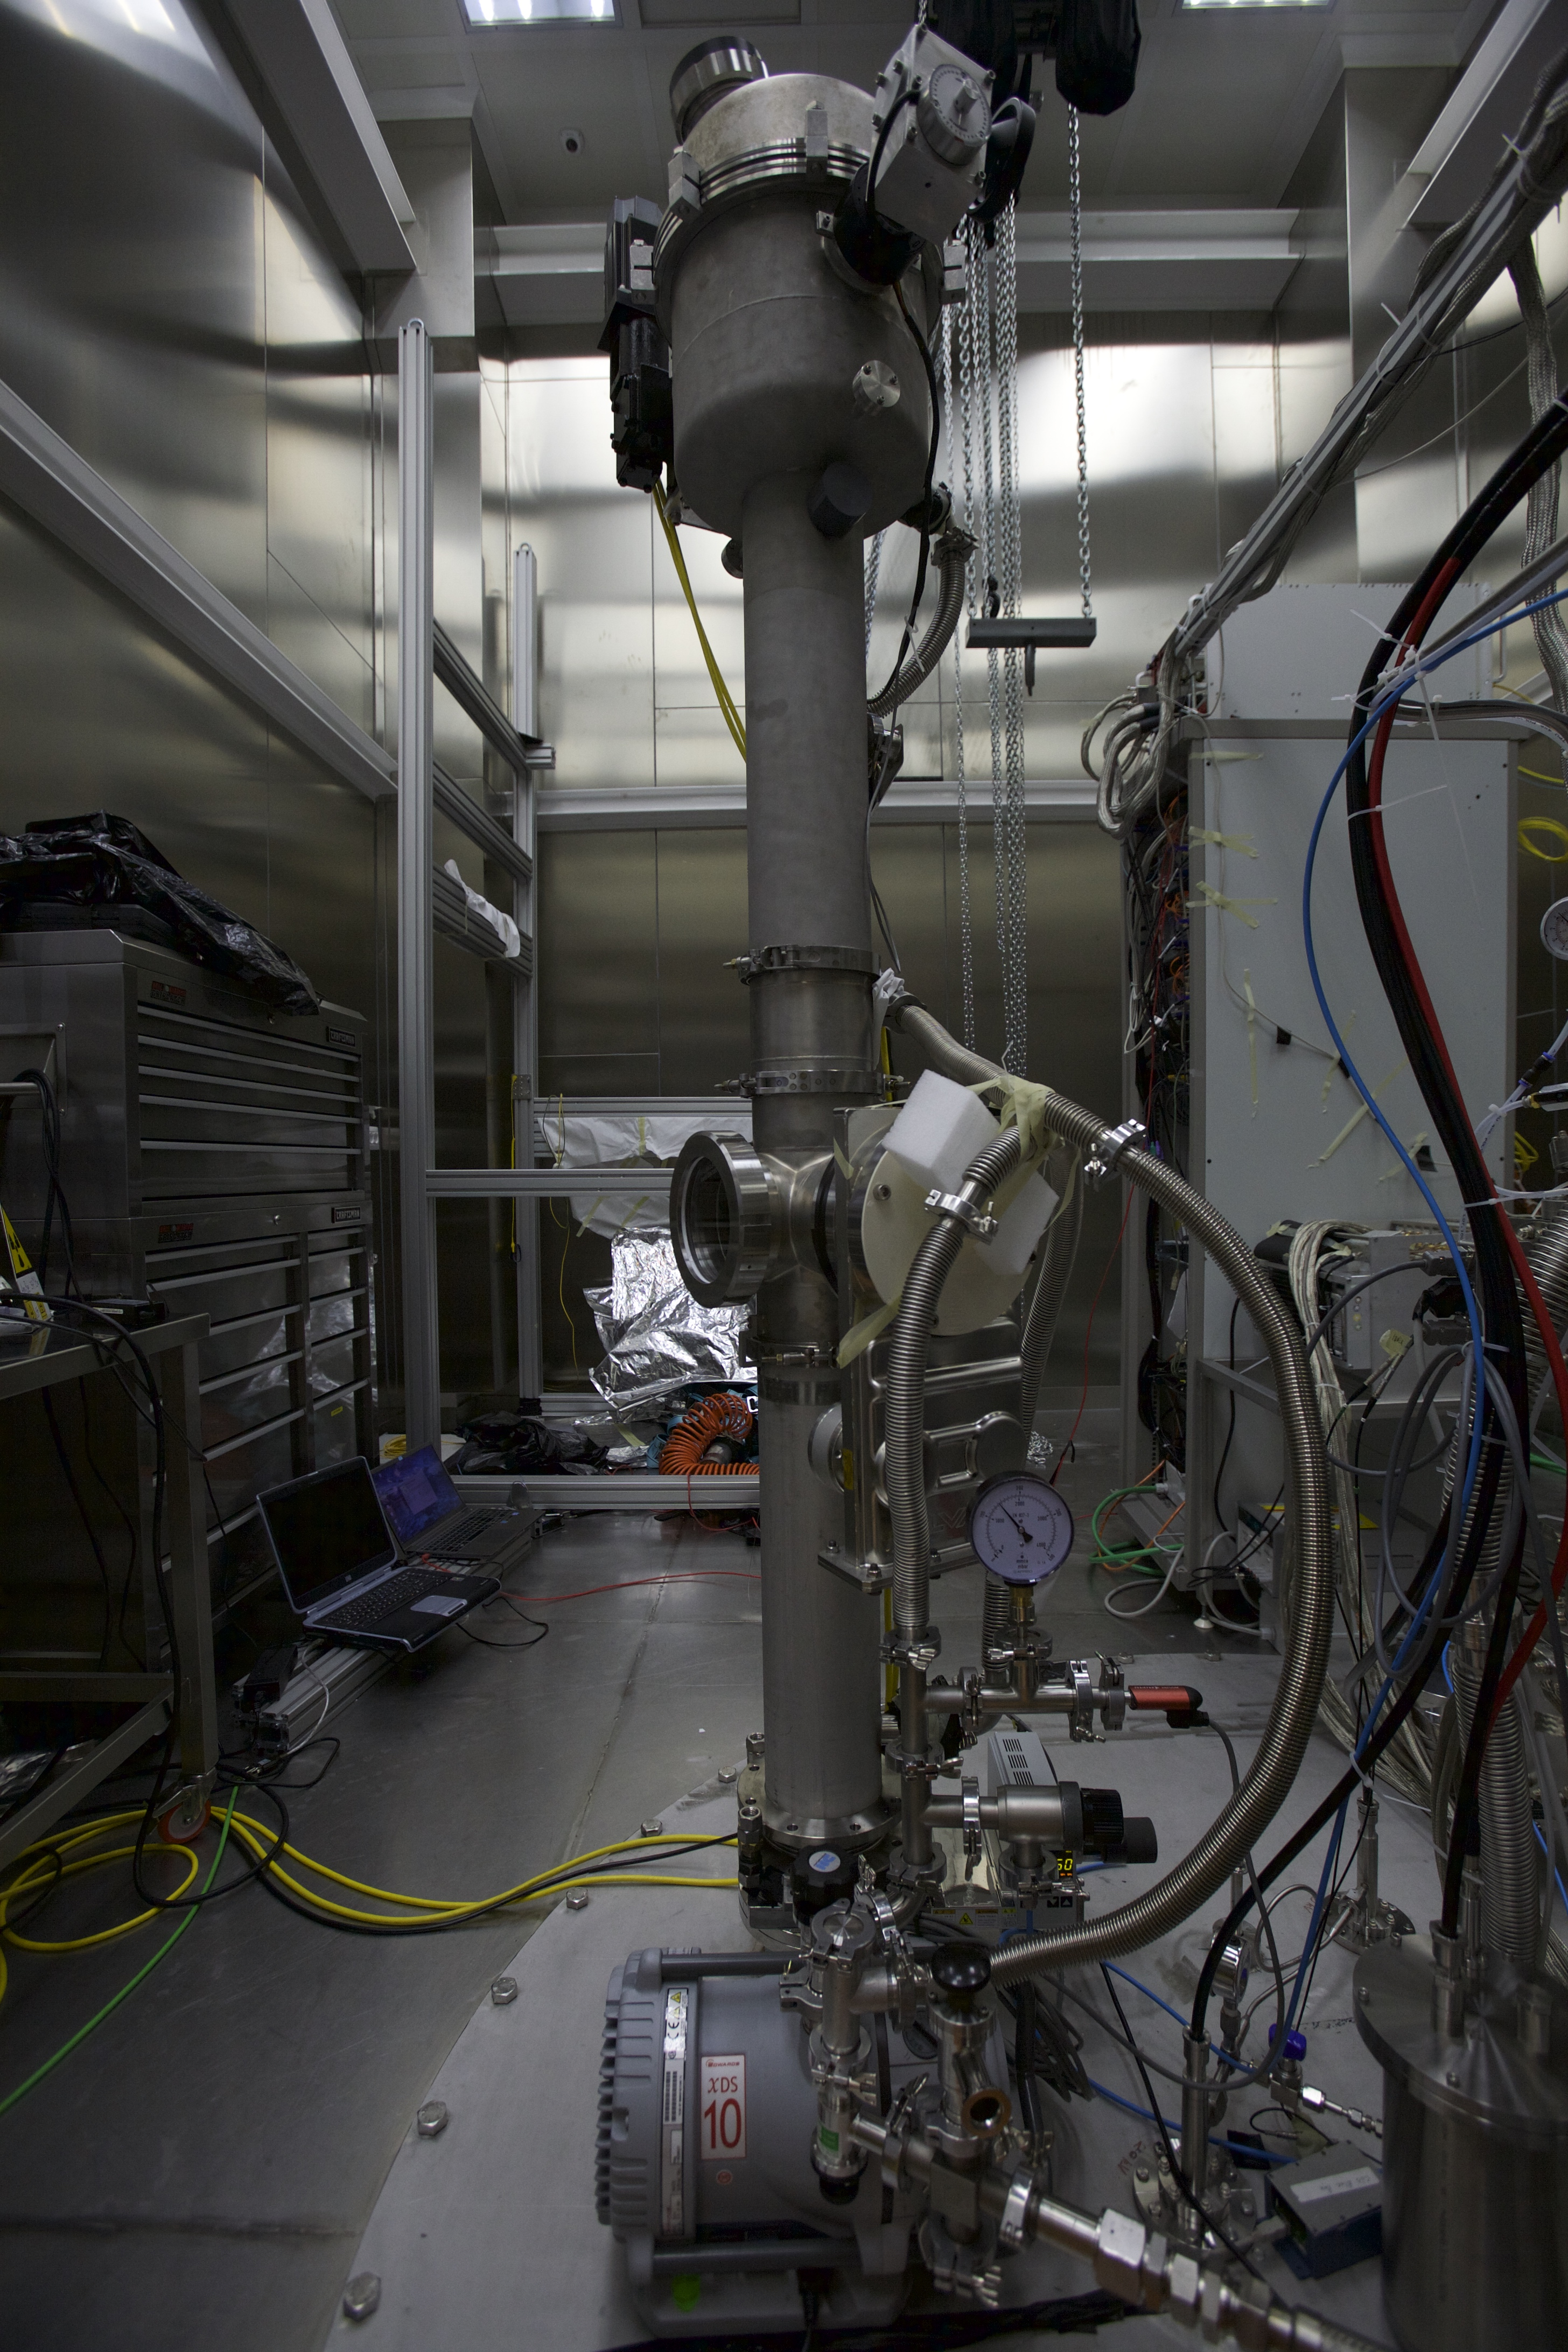
\includegraphics[width=0.49\textwidth]{Figures/CALIS_Tubings_IMG_3763.JPG}
  \caption{flushing and nitrogen purging system.}
  \label{fig:flushing_purging}
\end{figure}




\paragraph{Opening the Gate Valve}
\subsubsection{Positioning of Source}
\paragraph{Contact with Cryostat}
\paragraph{Cameras}
\subsubsection{Source Retraction and Extraction}
The source may not get in contact with the liquid scintillator. It is therefore sealed during the deployment in a dedicated source holder. In order to exchange sources the source arm and source holder has to be extracted from the pig into CRH and thereby comes in contact with normal air, containing oxygen and traces of water. After insertion a flush \& purge cycle is used to reduce, as known from glove boxes. No glove box present. Much more compact design.
% no glove box

After each deployment check that there is no leakage of Scintillator inside the source holder.



for what is helium leak tightness necessary? What was tested for helium leak tightness.



%tested for helium leak tightness

 
\section{Calibration Campaigns}\label{sec:CalibCampaigns}
\subsection{Radioactive Sources}
For the calibration of the LSV detector response and the TPC's response to electron recoils (ER) we selected $^{57}$Co, $^{133}$Ba and $^{137}$Cs. In a later calibration campaign also $^{22}$Na has been deployed. They allow a cross-calibration with $^{83m}$Kr, that has been injected in the Ar recirculation system during dedicated campaigns and the internal $^{39}$Ar, as they cover the energy range of $^{39}$Ar (see also Table~\ref{tbl:GammaSources} and Fig.~\ref{fig:GammaSources_Ar39spectrum}). %As the interaction length increases with energy in LAr, the different gamma sources allow also to probe different regions of the TPC active volume.  
\mymarginpar{possible upgrade for fig.16: all measured spectra overlayed at a fixed HV: 83mKr, Co57, Ba133, Cs137 (either null field or 200 V/cm) - ask Brianne? Also for her thesis?}

After a preselection of gamma source energies, detailed studies with the DarkSide Monte Carlo simulation package G4DS \cite{DS50:G4DS:paper} were performed to select appropriate source activities and check the feasibility and physics reach of various deployment positions. Considering also constraints from the LSV and TPC DAQs, sources with suitable activities were identified for deployment (Table~\ref{tbl:GammaSources}).

Energy variables are calibrated in photo-electrons (PE) using dedicated Laser calibration runs, in which the single PE charge spectra for each PMT are fitted and a PE-charge gain is determined. 
These Laser runs are also an integral part of a calibration campaign requiring a Laser run every few hours and at least on each change in DAQ or CALIS configuration, such as drift field changes or source position changes.

\begin{figure}[htbp]
 \centering
 \includegraphics[width=0.8\textwidth]{Figures/GammaSources_Ar39spectrum.png}
 \caption{Scintillation spectrum (S1) at null field showing a $^{83m}$Kr peak on the $^{39}$Ar $\beta$ spectrum. The energies of the three gamma sources are indicated and cover the full range of the $^{39}$Ar spectrum.
\label{fig:GammaSources_Ar39spectrum}}
\end{figure}

\begin{table}[htbp]
\caption{Gamma sources deployed in DS-50, $^{39}$Ar and $83m$Kr \cite{lippincott-kr}. Interaction length is in LAr. Activity of $^{39}$Ar has been approx. 50 Hz during AAr filling and negligible in the UAr phase. The Kr source activity varied from campaign to campaign, but was in the range of a few Bq to some tens of Bq.} %\cite{Lippincott:83mKr}
\centering
\begin{tabular}{|l|l|l|l|l|l|}
\hline
\textbf{source} & \textbf{type} & \textbf{energy} & \textbf{half life} & \textbf{interact. length} & \textbf{activity} \\ \hline
$^{57}$Co & $\gamma$ & 122 keV & 0.744 y & 4.4 cm & 35 kBq \\ \hline
$^{133}$Ba & $\gamma$ & 356 keV & 10.54 y & 7.5 cm & 2 kBq \\ \hline
$^{137}$Cs & $\gamma$ & 662 keV & 30.2 y & 9.5 cm & 0.65 kBq \\ \hline
$^{22}$Na & $\gamma$ & $2\cdot 511$ keV + 1274 keV & xxx y & xxx cm & 11 kBq \\ \hline\hline
$^{39}$Ar & $\beta$ &  565 keV endpoint& xxx y & sub-mm & 50 Hz \\ \hline
$^{83m}$Kr & 2 $\beta$ &  32.1 keV + 9.1 keV & xxx y & sub-mm & \\ \hline

\end{tabular}
\label{tbl:GammaSources}
\end{table}
\mymarginpar{get the numbers for Na22 in the table}

\subsection{Timeline of the Calibration Campaigns and Stability}
Between October 2014 and April 2016 the following calibration campaigns have been performed:
\begin{itemize}
\item The first extensive campaign involving all gamma sources and both the high and low activity AmBe neutron source took place in October and November 2014 at LNGS. The TPC was filled with Atmospheric Argon\mymarginpar{has atmospheric argon been introduced and underground argon?} with an inherent trigger rate of approx. 50 Hz from $^{39}$Ar. The liquid scintillator of the \lsv contained a PC only scintillator with $<0.1 \%$ TMB and 1.4 g/l PPO as wavelength shifter.
%Fig.~\ref{???} shows the different configurations in which data has been taken as a function of source energy, source position and drift field.

\item In January and February 2015 a second campaign focusing on the LSV calibration using the low activity AmBe source was performed. Prior to that the LSV has been reconstituted with 5 \% TMB\mymarginpar{what does 5 \% TMB mean? weight \%, volume \%?}. Two deployments were performed at two different PPO concentrations (0.7 g/l and 1.4 g/l), allowing to study the impact of the PPO concentration on alpha and gamma quenching. (1.4 g/l is our nominal PPO concentration, see also Fig.~\ref{fig:LSV:Calib}, right)

\item In August 2015 a $^{22}$Na source has been deployed next to the cryostat for TPC calibration. This was the first gamma source calibration campaign after the UAr deployment within \dsf.
\item In December 2015 an $^{241}$Am$^{13}$C neutron source has been deployed, allowing an in-depth study of the detection efficiency of the prompt neutron recoil signal in the absence of the correlated 4.4 MeV gamma, obfuscating the neutron recoil signal in case of an AmBe source.
\end{itemize}

As shown in Fig.~\ref{fig:LSV:Stability}\mymarginpar{instead of the timeline by Yann (DocDB 1232) I would like to show the Co60 and a rate stability plot - in progress.} the calibration campaigns have not affected negatively the light yield or introduced radioactivity into the LSV.

\begin{figure}[htbp]
\centering
\includegraphics[width=0.7\textwidth]{./Figures/Yann_timeline.png}
\caption{In black the stability of the LSV LY is monitored using internal $^{60}$Co emitted from the cryostat steel, in blue the stability of the rate of radioactivity in the LSV is shown. Before and after calibration campaigns both the LY and the rate remain unaffected.
\label{fig:LSV:Stability}}
 \end{figure}


\subsection{TPC Calibration}
A few calibration results are shown to illustrate the quality of the acquired calibration data and their description in G4DS \cite{DS50:G4DS:paper}.

\subsubsection{$^{57}$Co S1 energy}
Fig.~\ref{fig:CalibData:Co57} shows a data-MC comparison of the scintillation signal S1 spectrum of a $^{57}$Co calibration source deployed next to the cryostat and close to the TPC active volume center. Overlayed is the S1 distribution from an equivalent selection of G4DS MC simulation.\mymarginpar{The plot is from Paolo's G4DS talk \@ DS2016, UCLA. Ideally one could get an official copy from the MC paper.}

\begin{figure}[htbp]
\centering
\includegraphics[width=0.7\textwidth]{./Figures/57Co_Paolo_G4DS_UCLA.png}
\caption{Data-MC comparison for the $^{57}$Co source deployed next to the cryostat. In the magenta distribution a single-site interaction requirement has been imposed as for dark matter events and for the blue distribution this constraint has been removed \cite{DS50:G4DS:paper}.
\label{fig:CalibData:Co57}}
 \end{figure}


\subsubsection{F90 distribution from $^{241}$Am$^9$Be neutron data}\label{sec:CalibData:NR}

Fig.~\ref{fig:CalibData:F90} shows good agreement between F90 medians and S1 spectra measured from $^{241}$Am$^9$Be neutron data and those derived from \SCENE\ measurements, which have been used to determine the nuclear recoil energy scale and NR acceptance regions for the WIMP dark matter search \cite{ds:ds-50-PLB, DS:2ndPaper}.
\begin{figure}[htbp]
\centering
\includegraphics[width=0.7\textwidth]{./Figures/DSf-UArAmBeDMSStCut.pdf}
\caption{Plot of F90 vs. scintillation signal S1 from a high rate AmBe neutron source calibration of \dsf\ in grey, the upper NR band from the AmBe calibration and lower ER band from $\beta$-$\gamma$ backgrounds are visible. Overlayed are \FNinety\ \NR\ median vs. \SOne\ from a high-rate {\it in situ} AmBe\ calibration (blue) and scaled from \SCENE\ measurements (red points) \cite{scene2}. There is very good agreement between the two.  The high source intensity and correlated neutrons and $\gamma$-ray emission by the AmBe source contribute events outside the nuclear recoil and electron recoil bands. (reproduced from \cite{DS:2ndPaper})\label{fig:CalibData:F90}\label{fig:DSf-UArAmBeDMS}} 
\end{figure}


\subsubsection{Source position}
Tests at LNGS established the deployment system's positioning accuracy to be about $\pm$1 cm after a 7 meter journey into the DarkSide-50 \lsv.
%comment to the "about $\pm ": the tilde $~ \pm$ did not show up at all in the output.
During the first calibration campaign several runs have been taken with the source at its central position (731000 motor step counts). Fitting the t$_{drift}$ distribution at that position for a sequence of runs a systematic shift vs.~time has been observed (Fig.~\ref{fig:SourcePosition}, right). The source position has been on average 157.4 mm below the grid with an RMS of 10.1 mm. Following that observed systematic shift with time the deployment procedures have been revised to avoid such a time dependency in the future and to improve the deployment precision. It is worth mentioning though that this does not induce significant uncertainties for calibration data analyses, as the t$_{drift}$ distribution can be measured in-situ on a per-run basis and hence does not affect our dark matter analysis.
\begin{figure}[htbp]
\centering
\includegraphics[width=0.48\textwidth]{./Figures/Tdrift_distribution_Co57_DocDB1288.png}
\includegraphics[width=0.48\textwidth]{./Figures/SourcePosition_vs_time_DocDB1288.png}
\caption{\textit{left:} A t$_{drift}$ distribution encoding the z-position of the $^{57}$Co deployed next to the TPC center.
\textit{right:} Shift of source position relative to the TPC grid as a function of time when deployed to the same place.
\label{fig:SourcePosition}} 
\end{figure}

For the XY position the distribution of the azimuthal angle in the XY plane has been studied and a mean of 139 degrees has been observed with an RMS of 1.2 deg. (One degree corresponds to 6 mm at the outer cryostat, where the source is positioned.) However an independent XY reconstrution algorithm gave 142.5 degrees with an RMS of 0.8 deg, so that systematic uncertainties from the reonstruction dominate over the XY precision \cite{DS:XY:paper}.\mymarginpar{This is from DocDB 1288. Ideally one could cite a XY paper here, which is not published yet.}


%%%%%%%%%%%%%%%%%%%%%%%%%%%%%%%%

\subsection{Liquid Scintillator Veto}\label{sec:LSV:gammasources}

In Fig.~\ref{fig:LSV:Calib} (left) a data-MC comparison of the LSV charge spectra from the $^{137}$Cs source deployed in the LSV next to the cryostat is shown \cite{DS50:G4DS:paper}.
In January and February 2015 the reconstitution of the LSV scintillator was completed and a second AmBe neutron source calibration of the LSV calibration was undertaken to further study the various neutron detection channels in the LSV. With a borated scintillator, a critical aspect of the neutron detection efficiency is the capability to observe the \brbortenground\
capture branch leading to a \enbortengroundalpha\ $\alpha$ + $^7$Li(g.s.) without the accompanying 478 keV $\gamma$-ray. As shown in Fig.~\ref{fig:LSV:Calib} (right) the de-excitation channel is clearly observed at around 30 PE.

\begin{figure}[htbp]
\centering
\includegraphics[width=0.48\textwidth]{./Figures/137Cs_Veto_Paolo_G4DS_UCLA.png}
\includegraphics[width=0.48\textwidth]{./Figures/AmBe_LSV_VetoPaper.png}
\caption{\textit{left:} Data-MC comparison of the LSV charge spectra from the $^{137}$Cs source deployed in the LSV next to the cryostat \cite{DS50:G4DS:paper}.
\textit{right:} Clear detection of the neutron capture signal on $^{10}$B in the LSV leading to a \enbortengroundalpha\ $\alpha$ + $^7$Li(g.s.) at $\approx$ 30 PE (orange box). The
peak on the right at $\approx$ 270 PE (green box) is from the 93.6 \% of captures that lead to the $^7$Li excited state reaction, with the accompanying 478 keV-ray. The entries below 10 PE are due to PMT after-pulses. Data has been taken before and after varying the concentration of the wavelength shifter PPO in the scintillator with the source rotated 70 cm away from the cryostat. In both cases the deexcitation to ground state is clearly observed.\cite{DS50:VetoPaper}
\label{fig:LSV:Calib}} 
\end{figure}


\section{Analysis}\label{sec:analysis}

\subsection{TPC}

\subsubsection{$^{57}$Co S1 energy}
Fig.~\ref{fig:CalibData:Co57} shows a comparison of the scintillation signal S1 spectrum of a $^{57}$Co calibration source data deployed next to the cryostat and close to the TPC active volume center. Overlayed is the S1 distribution from an equivalent selection of G4DS MC simulation. Besides passing basic cuts like baseline found or all electronics channels present, the events were restricted to single-site interactions having one S1 and one S2 pulse, also the $^{39}$Ar background has been subtracted statistically. In the MC instead of an electronics simulation a clustering algorithm has been applied, that groups individual energy deposits and sums up the corresponding number of PE. A single-cluster cut has been applied to correspond to single-site interactions. The $^{57}$Co gamma ray spectrum (122 keV) reaching the TPC is significantly distorted by having to pass through the stainless steel source holder, outer and inner cryostat and the copper field cage rings before reaching the TPC's active volume.  These effects are accounted for by the MC even though refinements in the material description will further improve the already encouraging data-MC agreement. 

\begin{figure}[htbp]
\centering
\includegraphics[width=0.6\textwidth]{./Figures/Co57_LArTPC_center.png}
\caption{Data-MC comparison for the $^{57}$Co source deployed next to the cryostat. While some improvements are yet to be made, the level of agreement between the simulation and the various complex features of the data is very encouraging.
%A lack of resolution in the MC is expected as smearing due to electronics and reconstruction effects are not taken into account in the MC. THIS DOES NOT MAKE SENSE
\label{fig:CalibData:Co57}}
 \end{figure}


\subsubsection{position distributions}
\begin{figure}[htbp]
\centering
\includegraphics[width=0.55\textwidth]{./Figures/Co57_tdrift_data_731000-center+25mm.png}
\includegraphics[width=0.43\textwidth]{./Figures/50kg_Assembly_4-1-13_section_annotated_2.JPG}
\caption{\textit{left}: Data-MC comparison for the t$_{drift}$ distribution of the $^{57}$Co source deployed next to the cryostat and close to the active volume center. 
\textit{right:} Schematics of the TPC (without inner and outer cryostat) showing in particular the field rings, that cause a characteristic wave in the t$_{drift}$ spectrum of $^{57}$Co, which is also reproduced in MC (left) \cite{DS50:first_paper}.
\label{fig:CalibData:Co57:t_drift}}
\end{figure}

The t$_{drift}$ distribution of $^{57}$Co in Fig.~\ref{fig:CalibData:Co57:t_drift} is the same run set and event selection as for the S1 spectrum in Fig.~\ref{fig:CalibData:Co57}. It nicely illustrates the impact that the field rings have on the distribution. Fig.~\ref{fig:CalibData:XY_distrib} shows XY distributions of $^{133}$Ba and $^{137}$Cs sources deployed touching the cryostat from the left and right, respectively, exemplarily out of a pool of possible XY distributions.

\begin{figure}[htbp]
\centering
\includegraphics[width=0.55\textwidth]{./Figures/XY_Cs137_200Vcm_run10247_10252.png}
\includegraphics[width=0.43\textwidth]{./Figures/XY_Ba133_driftHV200_run10041_10310_right.png}
\caption{Two examples of XY distributions of $^{137}$Cs (left) and $^{133}$Ba (right) calibration source runs with the sources touching the cryostat from the left ($^{137}$Cs) and right ($^{133}$Ba). The $^{39}$Ar background is not subtracted and fills the TPC uniformly.
\label{fig:CalibData:XY_distrib}}
\end{figure}



\subsubsection{$^{241}$Am$^9$Be neutron data}\label{sec:CalibData:NR}

\begin{figure}[htbp]
\centering
\subfigure{\includegraphics[width=0.51\textwidth]{./Figures/Co57_LArTPC_center.png}}
%\subfigure{\includegraphics[width=0.46\textwidth]{./Figures/F90_data_DocDB1075.png}}
\subfigure{\includegraphics[width=0.47\textwidth]{./Figures/nr_f90_fit_apr2015_v8.pdf}}
 \caption{\textit{left}: Data-MC comparison for the $^{57}$Co source deployed next to the cryostat. While some improvements are yet to be made, the level of agreement between the simulation and the various complex features of the data is very encouraging.
%A lack of resolution in the MC is expected as smearing due to electronics and reconstruction effects are not taken into account in the MC. THIS DOES NOT MAKE SENSE
%\textit{right}: Distribution of pulse shape discrimination parameter F90 vs.~ S1 from \ar\ in AAr, overlayed with calibration data from $^{57}$Co and $^{133}$Ba sources. Good agreement with  the internal $^{39}$Ar illustrates the consistency of the calibration data.
\textit{right:} Plot of F90 vs. scintillation signal S1 from a high rate AmBe neutron source calibration of \dsf.  The pink line shows the mean F90 for the nuclear recoil band, while the points in green show the F90 values scaled from SCENE measurements and used in our publication Ref.~\cite{ds:ds-50-PLB}. There is very good agreement between the two.  The high source intensity and correlated neutrons and $\gamma$-ray emission by the AmBe source contribute events outside the nuclear recoil and electron recoil bands. 
\label{fig:CalibData:F90}}
 \end{figure}


%Distributions of the F90 pulse shape parameter from $^{57}$Co and $^{133}$Ba gamma sources outside the LAr-TPC are in good agreement with those from the internal calibration provided by the \ar \, decays, demonstrating the good quality of the calibration data set (Fig.~\ref{fig:CalibData:F90}, right). 

%At the time of publication of our paper Ref. \cite{ds:ds-50-PLB},  neutron calibration data was not available.  Therefore the WIMP search box for nuclear recoils was set based on measurements of F90 in the SCENE experiment \cite{scene2}. Now, a preliminary analyses of AmBe neutron source exposures shown in Fig.~\ref{fig:CalibData:F90}, lower left proves the good agreement between the extrapolated SCENE results and actual \dsf\ data.  

The WIMP search box and nuclear recoil acceptance in our paper~\cite{ds:ds-50-PLB} were established
without the availability of neutron calibration data in \dsf.  
The mean F90 from the ScENE experiment~\cite{scene2} was scaled to the light yield of DarkSide-50, and the electron and nuclear recoil acceptance curves were determined from an analytic statistical model of the F90 distributions as a function of energy. While we have full confidence in this approach, the 
data taken in the calibration campaign with the Am-Be neutron source now allow it to be directly
verified.  The mean F90 for nuclear recoils in \dsf\ is found to agree closely with the corresponding
scaled ScENE results, as shown in Fig.~\ref{fig:CalibData:F90}, right). 
%The same figure also shows Fig.~\ref{fig:CalibData:F90}, right also shows that the data with the Am-Be source will give us the mean F90 for nuclear recoils at energies beyond those measured by ScENE. 
(The higher-than-optimal intensity of this AmBe source and its 
correlated neutron and gamma ray emissions contribute events in the plot outside the nuclear recoil and electron recoil bands.)

\subsubsection{Z and XY of source position}
Tests at LNGS established the deployment system's positioning accuracy to be about $\pm$1 cm after a 7 meter journey into the DarkSide-50 detector.
%comment to the "about $\pm ": the tilde $~ \pm$ did not show up at all in the output.

 %Our first results show that the source can be positioned after its 7 meter journey into the DarkSide-50 detector with an accuracy of $~ \pm $1 cm.


This result is being validated using calibration campaign data in an ongoing analysis. 


\subsection{Liquid Scintillator Veto}\label{sec:LSV:gammasources}

In January and February 2015 the reconstitution of the LSV scintillator was completed and a second AmBe neutron source calibration of the LSV calibration was undertaken to further study the various
neutron detection channels in the LSV. With a borated scintillator, a critical aspect of the neutron detection efficiency is the capability to observe the \brbortenground\
capture branch leading to a \enbortengroundalpha\ $\alpha$ + $^7$Li(g.s.) without the accompanying 478 keV $\gamma$-ray. Veto results are described in further detail below in Sec.~\ref{sec:veto}.



\subsection{Impact of Calibration Source Deployment on Stability and Radioactivity in LY}
\section{Conclusions}\label{sec:Conclusions}\label{sec:Conclusion}
CALIS is a simple, affordable and effective source deployment system that has been successfully used to deploy sources in the LSV and next to the TPC and to conduct several successful calibration campaigns.%No adverse effects on the LSV or TPC have been noticed.

%summarize that the LSV and TPC detector have not been negatively affected.
%that's a sentence for the summary: The critical contribution by CALIS is the neutron veto detection efficiency calibration using dedicated neutron sources
%neutron gun inside a dedicated deployment device currently under development (Section \ref{sec:Outlook}).
%Refer to the next generation DS-detector.
%\section{Epilogue}\label{sec:Epilogue}
%here I would list all upcoming DarkSide papers and how they are in relationship with each other. Since so many papers are in preparation I would find that %helpful. Even if it is not eventually put into the paper.

%%%%%%%%%%%%%%%%%%%%%%%%%%%%%%%%%%%%%
%%%%%%%%%%%%%%%%%%%%%%%%%%%%%%%%%%%%%

\section{Acknowledgements}\label{sec:Acknowledgements}
\mymarginpar{This is a verbatim copy from the veto paper - adjustments needed?}The DarkSide-50 Collaboration would like to thank LNGS laboratory and its staff for invaluable technical and logistical support. This report is based upon work supported by the US NSF (Grants PHY-0919363, PHY-1004072, PHY-1004054, PHY-1242585, PHY-1314483, PHY-1314507 and associated collaborative grants; grants PHY-1211308 and PHY-1455351), the Italian Istituto Nazionale di Fisica Nucleare (INFN), the US DOE (Contract Nos. DE-FG02-91ER40671 and DE-AC02-07CH11359), and the Polish NCN (Grant UMO-2012/05/E/ST2/02333). We thank the staff of the Fermilab Particle Physics, Scientific and Core Computing Divisions for their support. We acknowledge the financial support from the UnivEarthS Labex program of Sorbonne Paris Cit\'{e} (ANR-10-LABX-0023 and ANR-11-IDEX-0005-02) and from the S\~{a}o Paulo Research Foundation (FAPESP).
%\input{acknowledgments.tex}

%% The Appendices part is started with the command \appendix;
%% appendix sections are then done as normal sections
%% \appendix

%% \section{}
%% \label{}

%% If you have bibdatabase file and want bibtex to generate the
%% bibitems, please use
%%
%%  \bibliographystyle{elsarticle-num} 
%%  \bibliography{<your bibdatabase>}

%% else use the following coding to input the bibitems directly in the
%% TeX file.

\begin{thebibliography}{00}

%% \bibitem{label}
%% Text of bibliographic item
\bibitem{Faber}S.M.~Faber and J.S.~Gallagher, \myrefs{Ann. Rev. Astron. Astroph. {\bf 17}, 135 (1979)}{10.1146/annurev.aa.17.090179.001031}.
\bibitem{WMAP1}D.N.~Spergel et al., \myrefs{Ap. J. Supp. {\bf 148}, 175 (2003)}{10.1086/377226}.
\bibitem{napp}Committee on Elementary Particle Physics in the 21st Century of the National Academies of Science, {\it Revealing the Hidden Nature of Space and Time: Charting the Course for Elementary Particle Physics}, Page~118, National Academies Press, Washington, DC (2006).
\bibitem{goodman}M.W.~Goodman and E.~Witten, \myrefs{Phys. Rev. D {\bf 31}, 3059 (1985)}{10.1103/PhysRevD.31.3059}.
\bibitem{warp}P.~Benetti et al. (WARP Collaboration), \myrefs{Astropart. Phys. {\bf 28}, 495 (2008)}{10.1016/j.astropartphys.2007.08.002}.
\bibitem{ds:ds-10-run3}T.~Alexander et al. (\ds\ Collaboration), \myrefs{Astropart. Phys. {\bf 49}, 44 (2013)}{10.1016/j.astropartphys.2013.08.004}.
\bibitem{ds:uar-extraction}H.O.~Back et al., \arxiv{1204.6024}.
\bibitem{ds:uar-distillation}H.O.~Back et al., \arxiv{1204.6061}.
\bibitem{loosli}H.H.~Loosli, \myrefs{Earth Plan. Sci. Lett. {\bf 63}, 51 (1983)}{10.1016/0012-821X(83)90021-3}.
\bibitem{warp:39ar}P.~Benetti et al. (WARP Collaboration), \myrefs{Nucl. Inst. Meth. A {\bf 574}, 83 (2007)}{10.1016/j.nima.2007.01.106}.
\bibitem{ds:uar-counting}J.~Xu et al., \myrefs{Astropart. Phys. {\bf 66}, 53 (2015)}{10.1016/j.astropartphys.2015.01.002}.

\bibitem{ctf:results}G.~Alimonti et al. (Borexino Collaboration), \myrefs{Astropart. Phys. {\bf 8}, 141 (1998)}{10.1016/S0927-6505(97)00050-9}.
\bibitem{ctf:scitech}G.~Alimonti et al. (Borexino Collaboration), \myrefs{Nucl. Instr. Meth. A {\bf 406}, 411 (1998)}{10.1016/S0168-9002(98)00018-7}.
\bibitem{lngs-depth}G.~Bellini et al. (\bx\ Collaboration), \myrefs{JCAP {\bf 1308}, 049 (2013)}{10.1088/1475-7516/2013/08/049}.
\bibitem{bx:detector}G.~Alimonti et al. (Borexino Collaboration), \myrefs{Nucl. Instr. Meth. A {\bf 600}, 568 (2009)}{10.1016/j.nima.2008.11.076}.
\bibitem{bx:plants}G.~Alimonti et al. (Borexino Collaboration), \myrefs{Nucl. Instr. Meth. A {\bf 609}, 58 (2009)}{doi:10.1016/j.nima.2009.07.028}.
\bibitem{boulay}M.~G.~Boulay and A.~Hime, \myrefs{Astropart. Phys. {\bf 25}, 179 (2006)}{10.1016/j.astropartphys.2005.12.009}.
\bibitem{bx:7be-precision}G.~Bellini et al. (\bx\ Collaboration), \myrefs{Phys. Rev. Lett. {\bf 107}, 141302 (2011)}{10.1103/PhysRevLett.107.141302}.
\bibitem{bx:phase-I}G.~Bellini et al. (\bx\ Collaboration), \myrefs{Phys. Rev. D {\bf 89}, 112007 (2014)}{10.1103/PhysRevD.89.112007}.
\bibitem{daya-bay}F.P.~An et al. (Daya Bay Collaboration), \arxiv{1407.0275}.
\bibitem{lumirror}\url{http://www.toray.jp/films/en/properties/lumirror/lum\_e6sr.html}, archived at \url{https://web.archive.org/web/20110405061457/http://www.toray.jp/films/en/properties/lumirror/lum_e6sr.html}.
\bibitem{wright} A.~Wright, P.~Mosteiro, and F.~Calaprice, \myrefs{Nucl. Instr. Meth. A {\bf 644}, 18 (2011)}{10.1016/j.nima.2011.04.009}.
\bibitem{greenwood} L.R.~Greenwood and N.R.~Chellew, \myrefs{Rev. Sci. Instr. {\bf 50}, 466 (1979)}{10.1063/1.1135853}.
\bibitem{wang} S.C.~Wang et al., \myrefs{Nucl. Instr. Meth. A {\bf 432}, 111 (1999)}{10.1016/S0168-9002(99)00350-2}.
\bibitem{scene1}T.~Alexander et al. (SCENE Collaboration), \myrefs{Phys. Rev. D {\bf 88}, 092006 (2013)}{10.1103/PhysRevD.88.092006}.
\bibitem{scene2}T.~Alexander et al. (SCENE Collaboration), \arxiv{1406.4825}.  Note that in Column 2 of our Table \ref{tab:scene}, we need $\mathcal{L}_{\rm eff,\,\krthree}$ for \dsfdriftfield, that is, the nuclear recoil light yield at \dsfdriftfield\ divided by the  \krthree\ at zero field.  This is not tabulated in the \scene\ paper.  (Table II of this reference gives $\mathcal{L}_{\rm eff,\,\krthree}$ at zero field.)  For our Table \ref{tab:scene}, we use the \dsfdriftfield\ data plotted in Fig.~8 of this reference.
\bibitem{saes}\mref{www.saesgetters.com}, archived at \url{https://web.archive.org/web/20141222175229/http://www.saesgetters.com/}.
\bibitem{venos}D.~V\'enos, A.~\v{S}palek, O.~Lebeda, M.~Fi\v{s}er, \myrefs{Appl. Rad. Isotopes {\bf 63}, 323 (2005)}{10.1016/j.apradiso.2005.04.011}.
\bibitem{lippincott-kr}W.H. Lippincott, S.B.~Cahn, D.~Gastler, L.W.~Kastens, E.~Kearns, D.N.~McKinsey, and J.A.~Nikkel, \myrefs{Phys. Rev. C {\bf 81}, 045803 2010)}{10.1103/PhysRevC.81.045803}.
\bibitem{kubota}S.~Kubota, M.~Hishida, and A.~Nohara, \myrefs{Nucl. Instr. Meth. {\bf 150}, 561, (1978)}{10.1016/0029-554X(78)90128-3};
M.J.~Carvalho and G.~Klein, \myrefs{J. Lumin. {\bf 18-19}, 487 (1979)}{10.1016/0022-2313(79)90167-4};
J.W.~Keto, R.E.~Gleason, and F.K. Soley, \myrefs{J. Chem. Phys. {\bf 71}, 2676 (1979)}{10.1063/1.438625};
T.~Suemoto and H.~Kanzaki, \myrefs{J. Phys. Soc. Japan {\bf 46}, 1554 (1979)}{10.1143/JPSJ.46.1554};
S.~Kubota, M.~Hishida, M.~Suzuki, J-z.~Ruan, \myrefs{Nucl. Instr. Meth. {\bf 196}, 101 (1982)}{10.1016/0029-554X(82)90623-1};
S.~Kubota et al., \myrefs{Phys. Rev. B {\bf 20}, 3486 (1979)}{10.1103/PhysRevB.20.3486}.
\bibitem{hitachi}A.~Hitachi, T.~Takahashi, N.~Funayama, K.~Masuda, J.~Kikuchi, and T.~Doke, \myrefs{Phys. Rev. B {\bf 27}, 5279 (1983)}{10.1103/PhysRevB.27.5279}.
\bibitem{doke} E.~Shibamura, K.~Masuda, and T.~Doke, Research Report to the Ministry of Education, Science, Sport, and Culture for Grant-in-Aid Scientific Research(C), No.~62540284 (1988).
\bibitem{xenon93}P.~Benetti et al., \myrefs{Nucl. Instr. Meth. A {\bf 327}, 203 (1993)}{10.1016/0168-9002(93)91442-P}.
\bibitem{ds:daq}P.~Agnes et al. (\ds\ Collaboration), \arxiv{1412.2969}.
\bibitem{caen}\mref{www.caen.it}, archived at\newline  \url{https://web.archive.org/web/20150104083159/http://www.caen.it/}.
\bibitem{ni}\mref{www.ni.com}, archived at\newline  \url{https://web.archive.org/web/20150218101935/http://www.ni.com/}.
\bibitem{highland}\mref{www.highlandtechnology.com}, archived at \url{https://web.archive.org/web/20150215110202/http://www.highlandtechnology.com/}.
\bibitem{art} C.~Green et al., \myrefs{J. Phys. Conf. Ser. {\bf 396}, 022020 (2012)}{10.1088/1742-6596/396/2/022020}.
\bibitem{empl}A.~Empl, R.~Jasim, E.V.~Hungerford, and P.~Mosteiro, \myrefs{JCAP {\bf 1408}, 64 (2014)}{10.1088/1475-7516/2014/08/064}.
\bibitem{deap-pollmann} T.~Pollmann, M.~Boulay, and M.~Kuzniak, \myrefs{Nucl. Instrum. Meth. A {\bf 635}, 127 (2011)}{10.1016/j.nima.2011.01.045}.
\bibitem{pocar} A.~Pocar, {\it Low Background Techniques and Experimental Challenges for Borexino and its Nylon Vessels}, Ph.D. Dissertation, Princeton University (2003).  \mref{search.proquest.com/docview/288218433/abstract}.
\bibitem{bx-vessels}J.~Benziger et al., \myrefs{Nucl. Instr. Meth. A {\bf 582}, 509 (2007)}{10.1016/j.nima.2007.08.176}.
\bibitem{sno-ncd}B.~Aharmim et al. (SNO Collaboration), \myrefs{Phys. Rev. Lett. {\bf 101}, 111301 (2008)}{10.1103/PhysRevLett.101.111301}.
\bibitem{lippincott}W.H.~Lippincott, K.~J.~Coakley, D.~Gastler, A.~Hime, E.~Kearns, D.N.~McKinsey, J.A.~Nikkel, and L.C.~Stonehill, \myrefs{Phys. Rev. C {\bf 78}, 035801 (2008)}{10.1103/PhysRevC.78.035801}.  Note that there is a misprint in the relevant equation 11.
\bibitem{deap}M.G.~Boulay et al. (DEAP Collaboration), \arxiv{0904.2930}.
\bibitem{lewin}J.D.~Lewin and P.~Smith, \myrefs{Astropart. Phys. {\bf 6}, 87 (1996)}{10.1016/S0927-6505(96)00047-3}.
\bibitem{savage}C.~Savage, K.~Freese, and P.~Gondolo, \myrefs{Phys. Rev. D {\bf 74}, 043531 (2006)}{10.1103/PhysRevD.74.043531}.
\bibitem{smith}M.C.~Smith et al., \myrefs{Mon. Not. Roy. Astron. Soc. {\bf 379}, 755 (2007)}{10.1111/j.1365-2966.2007.11964.x}.
\bibitem{gelmini}C.~Savage, G.~Gelmini, P.~Gondolo, and K.~Freese, \myrefs{JCAP {\bf 0904}, 010 (2009)}{10.1088/1475-7516/2009/04/010}.
\bibitem{lux}D.S.~Akerib et al. (LUX Collaboration),\myrefs{Phys. Rev. Lett. {\bf 112}, 091303 (2014)}{10.1103/PhysRevLett.112.091303}.
\bibitem{xenon-100}E.~Aprile et al. (XENON100 Collaboration), \myrefs{Phys. Rev. Lett {\bf 109}, 181301 (2012)}{10.1103/PhysRevLett.109.181301}.
\bibitem{pandax-i}M.~Xiao et al. (PandaX Collaboration), \arxiv{1408.5114}.
\bibitem{cdms}Z.~Ahmed et al. (CDMS II Collaboration), \myrefs{Science {\bf 327}, 1619 (2010)}{10.1126/science.1186112}.


\end{thebibliography}
\end{document}
\endinput
%%
%% End of file `elsarticle-template-num.tex'.
